% !TEX root = ../thesis-example.tex
%

\chapter{Real-time Ultrasound Uncertainty Estimation}
\label{chap:cudacm}

As with every kind of information, also medical images carry uncertainty, which should always be taken into account in order to interpret them correctly.
The fact that uncertainty can be formed of many different facets and originate from various sources makes it a difficult \SYN{feature,quantity} to understand.
Thomson et al. categorize uncertainty into the nine different types of accuracy/error, precision, completeness, consistency, lineage, currency, credibility, subjectivity and inter-relatedness \cite{Thomson:2005:UncertaintyTopology}.
Some of these facets are directly based on the physics of the image acquisitions and can thus be estimated through mathematical models. 
Others are specific to the individual user, patient anatomy and other features, which can not be estimated directly.


With respect to B-mode ultrasound, the physics of the image formation process poses a significant source of uncertainty.
Ultrasound images exhibit a wide range of image artifacts and require a large amount of training in order to be interpreted correctly \cite{Aldrich:2007:USPhysics,Scanlan:1991:Artifacts}.
Thus, being able to estimate the amount of uncertainty present in an image is an important step to improve ultrasound imaging.
One major source of uncertainty is the presence of signal attenuation in terms of shadowing and dropout artifacts.
Different approaches have been presented to estimate the amount of signal loss and \SYN{use this knowledge} to improve the results of tasks such as segmentation, tissue characterization and image registration \cite{Noble:2010:Ultrasound, Noble:2011:Ultrasound}.
So far however, ultrasound uncertainty estimation has always been an offline task not integrating well with one of the key benefits of ultrasound imaging \SYN{of} being an interactive modality.
In this chapter we discuss and present a real-time capable method to estimate ultrasound signal attenuation from the B-mode images themselves (cf. Figure \ref{fig:cudacm:liver_us_cm}).
We therefore extend the original formulation of ultrasound Confidence Maps \cite{Karamalis:2012:ConfidenceMaps} by an incremental solver scheme and show \SYN{that the accuracy of the results is sufficient for real-time visual computing and visualization applications}.
Parts of this work have been published in \CN.

\section{The B-mode Ultrasound Image Formation Process}
\label{sec:cudacm:us-image-formation}
%\TODO{Discussion of the ultrasound image formation process and the resulting uncertainty. Use Christoph's thesis as inspiration.}

While the general term of ultrasound describes the entire frequency range of acoustic waves that are not perceivable by the human ear ($20$ KHz to $1$ GHz), ultrasound in the context of medical imaging is used as a synonym of the imaging modality using frequencies between $1$ and $60$ MHz.
Historically, the first works on understanding the fundamentals of ultrasound date back to the 18th century to the findings of Euler, Lagrange, Rayleigh and many others \cite{Cobbold:2007:UsFoundations,Brooks:2008:Ultrasound}.
From the technical point of view, a major step towards today's ultrasound machines was the discovery of the Piezo-electric effect \cite{Curie:1880:PiezoEffect}, allowing to transform mechanical stress into electric potentials and vice versa.
While early developments were only considering 1D transmission over time (A-mode (Amplitude) ultrasound), the key work towards 2D cross-sectional ultrasound imaging was the system of Wild and Reid \cite{Wild:1952:Application} as it introduced showing the amount of reflection as brightness and thereby shaping today's B-mode imaging.

\begin{figure}[ht]
	\centering
	\begin{tikzpicture}[
	thick, decoration={coil, aspect=0.3, amplitude=-10mm},
	wave/.style={
		decorate, decoration={segment length=4mm}
	},
	compr/.style={
		decorate, decoration={segment length=2mm}
	},
	rare/.style={
		decorate, decoration={segment length=8mm}
	},
]

	\draw[wave]  (0cm, 0) -- (2cm, 0);
	\draw[compr] (2cm, 0) -- (3cm, 0);
	\draw[wave]  (3cm, 0) -- (5cm, 0);
	\draw[wave, transform canvas={xscale=1.6}, semithick]  (3.125cm, 0) -- (4.375cm, 0);
	%\draw[rare]  (5cm, 0) -- (7.41cm, 0);
	\draw[wave]  (7cm, 0) -- (9cm, 0);
	\draw[compr] (9cm, 0) -- (10cm, 0);
	\draw[wave]  (10cm, 0) -- (12cm, 0);
	
	\node [fill=white] at (2.25cm, 0) { Compression };
	\node [fill=white] at (5.9cm, 0) { \ Rarefaction \ };
	\node [fill=white] at (9.25cm, 0) { Compression };
	
	\draw [pfeil, <->] (2.25, 1.25) to node [color=MyColor2, sloped, above] {$\lambda$} (9.25, 1.25);
\end{tikzpicture}
	\caption{
		Illustration of a \textbf{longitudinal wave} exhibiting compression and rarefaction.
	}
	\label{fig:cmvis:longitudinal-wave}
\end{figure}

The ultrasound image formation process starts with the transducer sending out a short ultrasound pulse sequence into the body.
This pulse propagates as longitudinal wave (cf. Figure \ref{fig:cmvis:longitudinal-wave}) through the tissues and gets partly absorbed and reflected at different depths until these echoes eventually reach the transducer again where they are recorded.
After several processing steps and assuming a constant speed of sound of $1540 \frac{\text{m}}{\text{s}}$, the intensity and runtime of the ultrasound echoes, representing reflectance and depth, can be used to form a 2D image of the underlying anatomy.

\begin{figure}[ht]
	\centering
	\begin{tikzpicture}[line join=round]
	% the transducer	
	\filldraw [color=black, fill=gray!25, semithick]
		(-10mm, 0cm) 
			to[rounded corners=0.2mm] (-10mm, 7mm) 
			to[rounded corners] (0mm, 9mm) 
			to[rounded corners] (15mm, 10mm) 
			to[rounded corners] (17mm, 15mm) 
			to[rounded corners] (25mm, 12mm) 
		-- (25mm, 0mm) 
			to[rounded corners] (25mm, -12mm) 
			to[rounded corners] (17mm, -15mm) 
			to[rounded corners] (15mm, -10mm) 
			to[rounded corners] (0mm, -9mm) 
			to[rounded corners=0.2mm] (-10mm, -7mm) 
		-- (-10mm, 0mm)
		;
	
	% Interface 1
	\draw [color=MyColor1, very thick, rounded corners, xshift=2cm]
		(44mm, 20mm) to (40mm, 17mm) to (39mm, 10mm) to (38mm, 5mm) to (40mm, 2mm) -- (40mm, -2mm) to (37mm, -12mm) to (40mm, -15mm) to (39mm, -18mm) to (41mm, -20mm);
	
	% Interface 2
	\draw [color=MyColor1, very thick, rounded corners, xshift=5cm]
		(43mm, 15mm) to (40mm, 10mm) to (39mm, 5mm) to (40mm, 2mm) -- (40mm, -2mm) to (41mm, -5mm) to (41mm, -12mm) to (44mm, -15mm);
	
	\node [color=MyColor1] at (64mm, 23mm) {Interface 1};
	\node [color=MyColor1] at (93mm, 18mm) {Interface 2};

	\node [color=black] at (42.5mm, -18mm) {$Z_1$};
	\node [color=black] at (75mm, -18mm) {$Z_2$};
	\node [color=black] at (105mm, -18mm) {$Z_3$};
	
	\draw [pfeil, line width=3pt] (25mm, 1.5mm) -- (60mm, 1.5mm);
	\draw [pfeil, line width=2pt] (60mm, -1.5mm) to (25mm, -1.5mm);
%	\draw [pfeil, line width=2pt] (60mm, -1.5mm) to node [sloped, below, color=MyColor2] {$R_1$} (25mm, -1.5mm);
	
	\draw [pfeil, line width=2pt] (60mm, 1.5mm) to (90mm, 1.5mm);
	\draw [pfeil, line width=1pt] (90mm, -1.5mm) to (60mm, -1.5mm);
	
	\draw [pfeil, line width=1pt] (90mm, 1.5mm) to (120mm, 1.5mm);
\end{tikzpicture}
	\caption{
		Simplified illustration of \textbf{reflection and transmission at tissue interfaces}.
		When an ultrasound wave crosses an interface between two tissues of different acoustic impedance, parts of the signal gets reflected while the remainder continues traveling through the anatomy (cf. Equation \ref{eq:cudacm:reflection-transmission-coefficients}).
	}
	\label{fig:cmvis:transducer-reflection}
\end{figure}

More precisely, the longitudinal ultrasound wave propagates areas of compression and rarefaction (cf. Figure \ref{fig:cmvis:longitudinal-wave}) through the anatomy inducing several different interactions with the tissue.
Within homogeneous media, the main \SYN{effect} is absorption where energy is dissipated over depth leading to a \SYN{mostly uniform} attenuation of the signal.
Furthermore, wave interference and diffraction, as well as further non-linear effects occur.
For diagnostic imaging however, the wave interactions with inhomogeneous media, namely reflection, transmission, refraction and scattering, are much more important.
Interfaces between two tissues of different acoustic impedance lead to a reflection of parts of the signal, while the remainder of the signal is further transmitted (cf. Figure \ref{fig:cmvis:transducer-reflection}), yielding a reflection coefficient $R_i$ and a transmission coefficient $T_i$:
\begin{equation}
	\label{eq:cudacm:reflection-transmission-coefficients}
	R_i	= \left( \frac{Z_2 - Z_1}{T_2 + Z_1} \right)^2, \quad
	T_i	= \frac{4Z_1 Z_2}{\left( Z_2 + Z_1 \right)^2}.
\end{equation}
According to Snell's law and the Fresnel equations, this reflection and transmission is angle dependent so that refraction \SYN{happens} and the direction of the longitudinal wave changes if an interface is not perpendicular to the wave front.
Since a tissue is never completely homogeneous, this process happens continuously and yields the characteristic ultrasound speckle patterns where the inhomogeneities are smaller than the wave length $\lambda$, often modeled as random point scattering.

This image formation process give B-mode ultrasound it's characteristic gradient-like appearance where the intensities rather show the changes in physical properties than the physical properties themselves.
In addition, these intensities are highly direction-dependent since the amount of observed reflection intensity decreases with increasing angle between sound direction and interface normal.
Thus, estimating signal attenuation and general uncertainty from B-mode image is a non-trivial task, for which different approaches have been presented \cite{Noble:2010:Ultrasound, Noble:2011:Ultrasound}.


\section{Confidence Maps for B-mode Ultrasound}
\label{sec:cudacm:cm}
%Introduce the concept of US Confidence Maps, and related work.

\begin{figure}[ht]
	\centering
	\subfloat[~Original liver ultrasound image.]{
		\label{fig:cudacm:liver_us}
		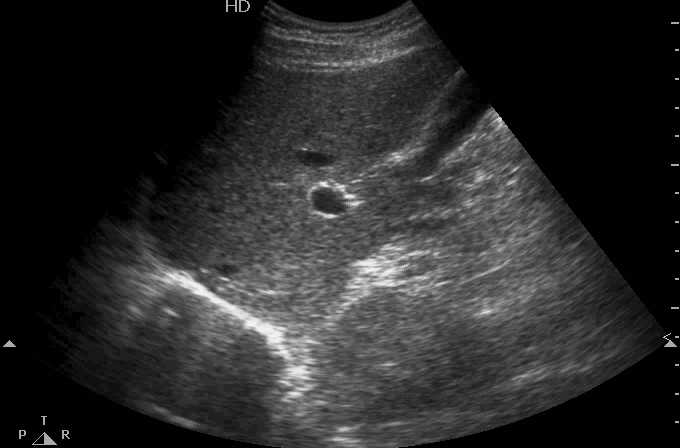
\includegraphics[width=0.47\linewidth]{figures/cudacm/liver_us.png}
	}
	\
	\subfloat[~Corresponding confidence map.]{
		\label{fig:cudacm:liver_cm}
		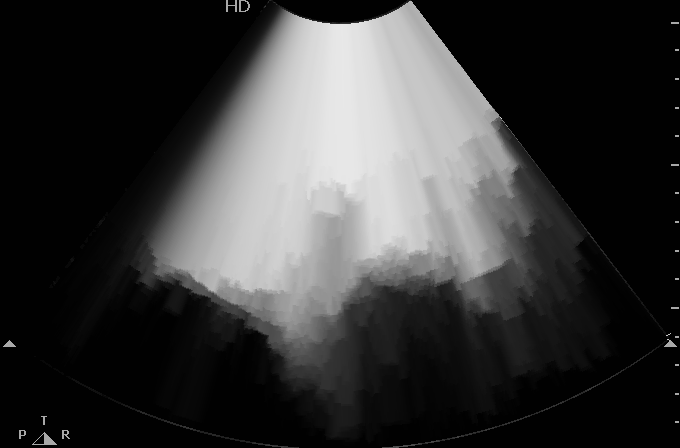
\includegraphics[width=0.47\linewidth]{figures/cudacm/liver_cm.png}
	}
	\caption{\textbf{Confidence maps on liver ultrasound}: (a) shows the original ultrasound image, (b) shows the corresponding confidence map, bright regions depicting regions of high confidence, dark regions depicting regions of low confidence.}
	\label{fig:cudacm:liver_us_cm}
\end{figure}

A \SYN{major} generalization of different concepts of ultrasound uncertainty estimation are ultrasound Confidence Maps, originally proposed by Karamalis et al. \cite{Karamalis:2012:ConfidenceMaps} and later refined by Hennersperger et al. \cite{Hennersperger:2014:EnergyMinimizationFramework}.
They describe a per-pixel estimation of the amount of uncertainty present in ultrasound images due to signal attenuation and shadowing, for which they employ a random walks formulation similar to the one by Grady to solve the $k$-label image segmentation problem \cite{Grady:2006:RandomWalks}.
Taking ultrasound physics into account, Confidence Maps describe the probability of a random walker starting from a given pixel to reach the virtual transducer elements.

\begin{figure}[ht]
	\centering
	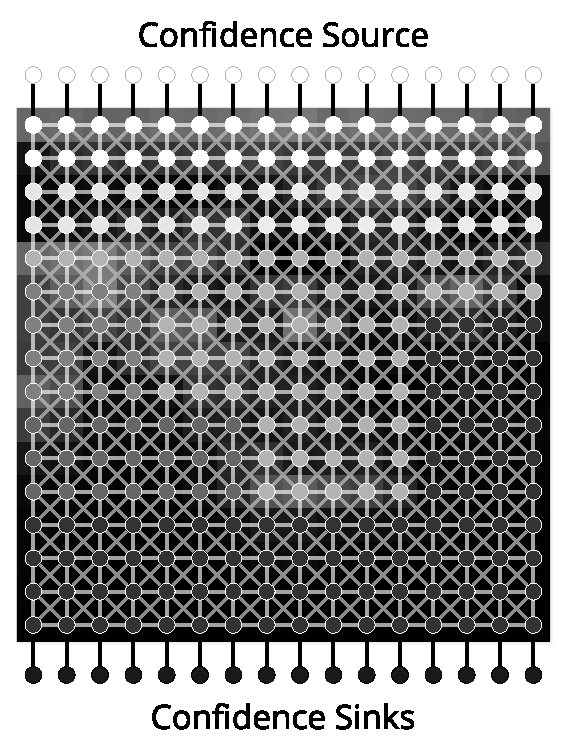
\includegraphics[width=0.5\linewidth]{./figures/cudacm/diffusion_problem_8n.pdf}
	\caption{Illustration of the \textbf{diffusion graph network for computing Confidence Maps}. Each node is connected to its 8 neighborhood where the edge weights are defined as a function of the edge direction and gradients in the B-mode image.}
	\label{fig:cudacm:diffusion-graph}
\end{figure}

As illustrated in Figure \ref{fig:cudacm:diffusion-graph}, the image is represented as an undirected graph $G = (V, E)$, where the nodes $v \in V$ represent the image pixels, each being connected to its 8 surrounding nodes through the edges $e \in E$.
Each edge $e_{ij} \in E$, connecting nodes $v_i$ and $v_j$ is assigned a weight $w_{ij} > 0$ describing the likelihood of the random walker crossing that edge.
Furthermore, a set of virtual transducer elements are placed at the start and end of each ultrasound scanline to define the signal attenuation boundary conditions.
The edge weights are given as
\begin{equation}
	\begin{split}
		w_{ij} &= 
			\begin{cases}
				\exp(-\beta (|c_i - c_j| + \gamma))         & \text{if $i, j$ adjacent and $e_{ij}$ horizontal edge} \\
				\exp(-\beta (|c_i - c_j|))                  & \text{if $i, j$ adjacent and $e_{ij}$ vertical edge}   \\
				\exp \left(-\beta (|c_i - c_j| + \sqrt 2 \gamma) \right) & \text{if $i, j$ adjacent and $e_{ij}$ diagonal edge}   \\
				0                                           & \text{otherwise},
			\end{cases} \\
		c_i &= g_i \exp(-\alpha l_i),
	\end{split}
\end{equation}
where $g_i$ is the image intensity at node $i$ and $l_i$ describes the normalized closest distance to the virtual transducer elements.
The three free parameters $\alpha, \beta$ and $\gamma$ define the \SYN{outcome} of the Confidence Maps.
While the $\alpha$ parameter describes the likelihood of random walks along vertical edges and thus scales the estimated  attenuation with increasing depth, $\beta$ affects the robustness and accuracy of the segmentation result.
Furthermore, $\gamma$ penalizes random walks along the horizontal and diagonal edges and thereby \SYN{adjusts} the amount of horizontal discontinuities.
A more thorough discussion of the edge weights and the free parameters can be found in the original paper \cite{Karamalis:2012:ConfidenceMaps}.
In their evaluation, Karamalis et al. demonstrate that ultrasound Confidenece Maps describe an accurate per-pixel estimate of the signal attenuation, which can be translated to the amount of uncertainty present in the image.
Typical applications are ultrasound shadow detection, 3D freehand ultrasound compounding and multi-modal registration.

Due to the formulation as diffusion problem with Dirichlet boundary conditions, where the scanline sources have full confidence and the scanline sinks have zero confidence, Confidence Maps always exhibit the whole value range of $[0, 1]$.
Thus, the computed values describe only relative information with respect to the current image.
As a consequence, one has to pay special attention when comparing Confidence Maps of different images.
While the values of images of the same sequence may be comparable, confidence values between images of different anatomies are not directly numerically comparable.


\section{Traditional Implementations}
%Short discussion on traditional implementations using direct solves, such as LU decomposition.

Due to the formulation as Dirichlet diffusion problem, the computation of ultrasound Confidence Maps can be efficiently encoded in a linear system of the form
\begin{equation}
	L \mathbf{x} = \mathbf{b},
	\label{eq:cudacm:cm-system}
\end{equation}
where $L$ describes the Laplacian matrix of the graph, $\mathbf{x}$ is the Confidence Map in vectorized form and $\mathbf{b}$ encodes the Dirichlet boundary conditions.
Since, the graph is undirected and describes an 8-neighborhood, $L$ is symmetric, sparse, and positive definite.
Thus, Equation \ref{eq:cudacm:cm-system} is traditionally be solved with direct methods such as LU decomposition \cite{Karamalis:2012:ConfidenceMaps}.

Unfortunately, direct solvers do not \SYN{suit well} the interactive \SYN{characteristic} of ultrasound imaging.
Even with the relatively moderate resolution of ultrasound images, real-time computation of Confidence Maps is not feasible with today's hardware.
Karamalis et al. report computation times of \SYN{a little more} than two seconds \cite{Karamalis:2012:ConfidenceMaps}, which was reproduced by our experiments.
Chatelain et al. use Confidence Maps for servoing of robotic ultrasound \cite{Chatelain:2015:UltrasoundServoing}.
However, in order to yield interactive frame rates they had to significantly downsample the ultrasound images and it is unclear how much this \SYN{impairs} the quality of the results.
Thus, other methods are needed in order to solve Equation \ref{eq:cudacm:cm-system} in real-time.


\section{Real-Time Incremental Solving}
In order to yield real-time Confidence Maps for our system, we leverage the dynamic nature of ultrasound acquisitions and the temporal coherency of its images based on the high acquisition rates of today's systems.
Consecutive images in ultrasound sequences usually differ very little and therefore the corresponding Confidence Maps will likely be very similar.
We exploit this fact by using an iterative Jacobi-preconditioned Conjugate Gradient solver instead of directly solving Equation \ref{eq:cudacm:cm-system} through matrix decompositions.
This allows us to execute an incremental computation scheme, where we directly use the resulting Confidence Maps as initialization for the subsequent frame (cf. Figure \ref{fig:cudacm:incremental-computation}). 
This greatly reduces the number of needed iterations per frame as we have a better convergence to the true solution in the limited time budget available per frame. 

\begin{figure}[ht]
	\centering
	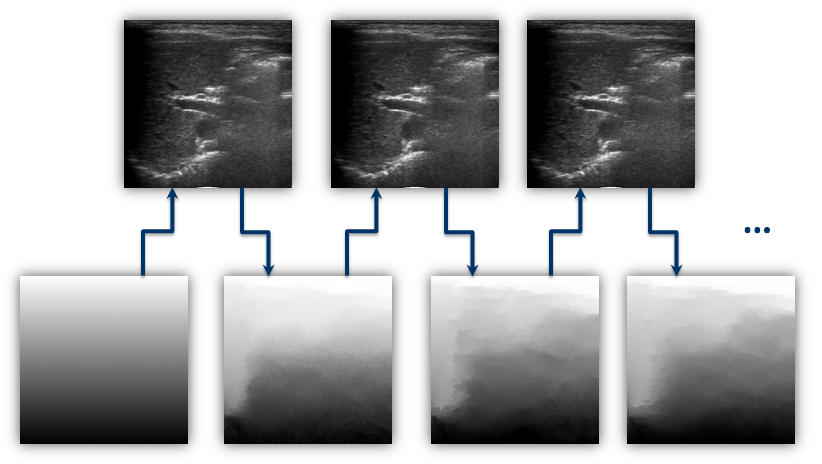
\includegraphics[width=0.75\linewidth]{./figures/cudacm/incremental-computation.png}
	\caption{Illustration of our proposed \textbf{incremental computation scheme} for Confidence Maps. Due to the temporal coherency of ultrasound imaging, consecutive images and thus also their Confidence Maps are usually very similar. Therefore, we use the each computed Confidence Map as initialization for the iterative solving of the subsequent frame.}
	\label{fig:cudacm:incremental-computation}
\end{figure}

We construct the equation system matrix $L$ explicitly on each frame.
Due to the given graph \SYN{layout}, the matrix has only 9 diagonals with non-zero entries and can thus be efficiently stored using the sparse DIA matrix storage format \CN.
For the very first frame, we initialize $x$ with a linear gradient as very rough approximation of the Confidence Map.
Then, for every subsequent frame, we use the computed result as initialization.
For easier integration with visualization techniques and to allow for an interactive experience in general, we implemented our technique on the GPU using CUDA.
The preconditioned Conjugate Gradient solver has a specific time budget depending on the target frame rate, in which it performs as many iterations as possible.
Even though this time budget might be too small to yield exact solutions from the beginning, our later evaluation shows, that the temporal coherency of ultrasound sequences is sufficient to have the solver converge within very few frames.

\begin{figure}[t]
	\centering
	\begin{tikzpicture}[
	schritt/.style={
		schritt-base, rectangle split, rectangle split parts=2, minimum height=8mm, minimum width=28mm
	},
	entity/.style={
		entity-base, minimum height=8mm, minimum width=22mm
	},
	portL/.style={
		font=\sffamily\scriptsize, outer xsep=1mm,
		align=left, anchor=west,
	},
	portR/.style={
		font=\sffamily\scriptsize, outer xsep=1mm,
		align=right, anchor=east,
	},
	pfeilkurz/.style={
		pfeil, shorten >=0.5mm
	},
	node distance=6mm and 10mm
	]

	\node (filter) [schritt] { \phantom{p}\textbf{Image Filter}\phantom{b} \nodepart{two}\\ };	
	\PORT{2L1}{($ (filter.two west) + (0, 0mm) $)}{MyColor2}{node[portL] {Input \phantom{pb}}}
	\PORT{2R1}{($ (filter.two east) + (0, 0mm) $)}{MyColor2}{node[portR] {\phantom{pb} Resampled US}}
%	\PORT{2R2}{($ (filter.two east) - (0, 2mm) $)}{MyColor2}{node[portR] {\phantom{pb} Blurred US}}

	\node (igtlink) [entity, left=of filter] {\textbf{US Image}};
	\PORT{1R1}{($ (igtlink.east) - (0mm, 0mm) $)}{MyColor2}{}
	
	\node (cmsolver) [schritt, right=of filter] { \textbf{Confidence Map Solver} \nodepart{two}\\\\ };	
	\PORT{4L1}{($ (cmsolver.two west) + (0, 2mm) $)}{MyColor4}{node[portL] {Initial Solution \phantom{pb}}}
	\PORT{4L2}{($ (cmsolver.two west) - (0, 2mm) $)}{MyColor2}{node[portL] {US Image \phantom{pb}}}
	\PORT{4R1}{($ (cmsolver.two east) + (0, 2mm) $)}{MyColor4}{node[portR] {\phantom{pb} CM}}

%	\node (ucmapping) [schritt, right=of cmsolver]{ \textbf{Uncertainty Mapping} \nodepart{two}\\\\\\\\ };	
%	\PORT{5L1}{($ (ucmapping.two west) + (0, 4mm) $)}{MyColor4}{node[portL] {CM \phantom{pb}}}
%	\PORT{5L2}{($ (ucmapping.two west) - (0, 0mm) $)}{MyColor2}{node[portL] {Blurred Image \phantom{pb}}}
%	\PORT{5L3}{($ (ucmapping.two west) - (0, 4mm) $)}{MyColor2}{node[portL] {B-mode US \phantom{pb}}}
%	\PORT{5R1}{($ (ucmapping.two east) + (0, 4mm) $)}{MyColor2}{node[portR] {\phantom{pb} Fused US}}

	\node (scanline) [entity, right=of cmsolver] { \textbf{Confidence Map} };
	\PORT{6L1}{($ (4R1) + (10mm, 0mm) $)}{MyColor4}{}
	
	
	\begin{pgfonlayer}{background}
		\draw [pfeilkurz] (1R1) to [out=0, in=180, in distance=6mm] (2L1);
%		\draw [pfeilkurz] (1R1) |- ($ (5L3) - (4mm, 6mm) $) |- (5L3);
	
		\draw [pfeilkurz] (2R1) to [out=0, in=180, in distance=6mm] (4L2);
%		\draw [pfeilkurz] (2R2) -| ($ (2R2) + (4mm, -4mm) $) |- ($ (5L2) - (6mm, 8mm) $) |- (5L2);
	
		\draw [pfeilkurz, draw=MyColor4] (4R1) -| ($ (4R1) + (3mm, 4mm) $) |- ($ (4R1) + (0mm, 11mm) $) -| ($ (4L1) + (-5mm, 4mm) $) |- (4L1);
%		\draw [pfeilkurz, draw=MyColor4] (4R1) -- ($ (4R1) + (3mm, 0mm) $) to ($ (5L1) - (5mm, 0mm) $) -- (5L1);
	
		\draw [pfeilkurz, draw=MyColor4] (4R1) -- (6L1);
	\end{pgfonlayer}{background}

\end{tikzpicture}
	\caption{
		\TODO{Redo this illustration to show only the cudacm parts, not the cmvis parts.}
		\textbf{Processing pipeline} of our reference implementation. We receive the original ultrasound B-mode image through OpenIGTLink and perform an Gaussian blur and a resampling in order to improve the PCG convergence performance. 
		The Confidence Map solver then incrementally computes the B-mode image's Confidence Map by using the previous image's Confidence Map as initialization. 
		Finally, we perform the uncertainty mapping using one of the three presented schemes (cf. Section \ref{sec:cmvis:mapping-schemes}) and transform the image from polar to cartesian coordinates.
	}
	\label{fig:cmvis:campvis_pipeline}
\end{figure}

As already discussed in Section \ref{sec:cudacm:cm}, Confidence Maps exhibit only a relative measure of confidence.
Their strength is not the exact confidence value at a single pixel, but rather the distribution within the image.
Thus, due to noise in the original ultrasound, the Confidence Maps of multiple consecutive frames may exhibit a flickering behavior when being watched in a sequence.
To introduce a better temporal coherency, we apply an additional alpha beta filter \cite{Brookner:1998:Filtering}.
Being a variant of the Kalman filter, it recursively operates on the stream of computed Confidence Maps and produces a smoothened version by averaging the current image with a prediction based on the previous images.
We empirically selected a configuration of $\alpha = 0.36$ and $\beta = 0.005$ providing good results with both damping of flickering and preservation of the original confidence distribution and temporal responsiveness of the estimates.


\section{Evaluation}
\label{sec:cudacm:evaluation-performance}
For the evaluation of our methods, we had a professional sonographer acquire several sequences of patient abdominal ultrasound.
Our system was run on a Linux notebook with an Intel i7 processor and a nVidia GTX 750M GPU. 
Instead of acquiring live images from the ultrasound machine, we streamed the pre-recorded sequences from the hard disk via OpenIGTLink link, each containing 392 images of 512x512 pixels resolution.
To examine the influence of the system performance with respect to the different parameters, we ran our real-time solver in various configurations.

\paragraph{Resample Scale vs. Number of Iterations}
The analytical solving of Equation \ref{eq:cudacm:cm-system} using standard Cholesky decomposition requires an average of more than 2.2 seconds per frame and is thus far from real-time.
In contrast, our proposed incremental solver scheme allows to stop the iteration process at any time and use the best possible solution that can be computed within a give time budget.
We set this to $30$ms in order to ensure real-time applications with a target frame of $30$ fps.
\begin{figure}[ht]
	\centering
	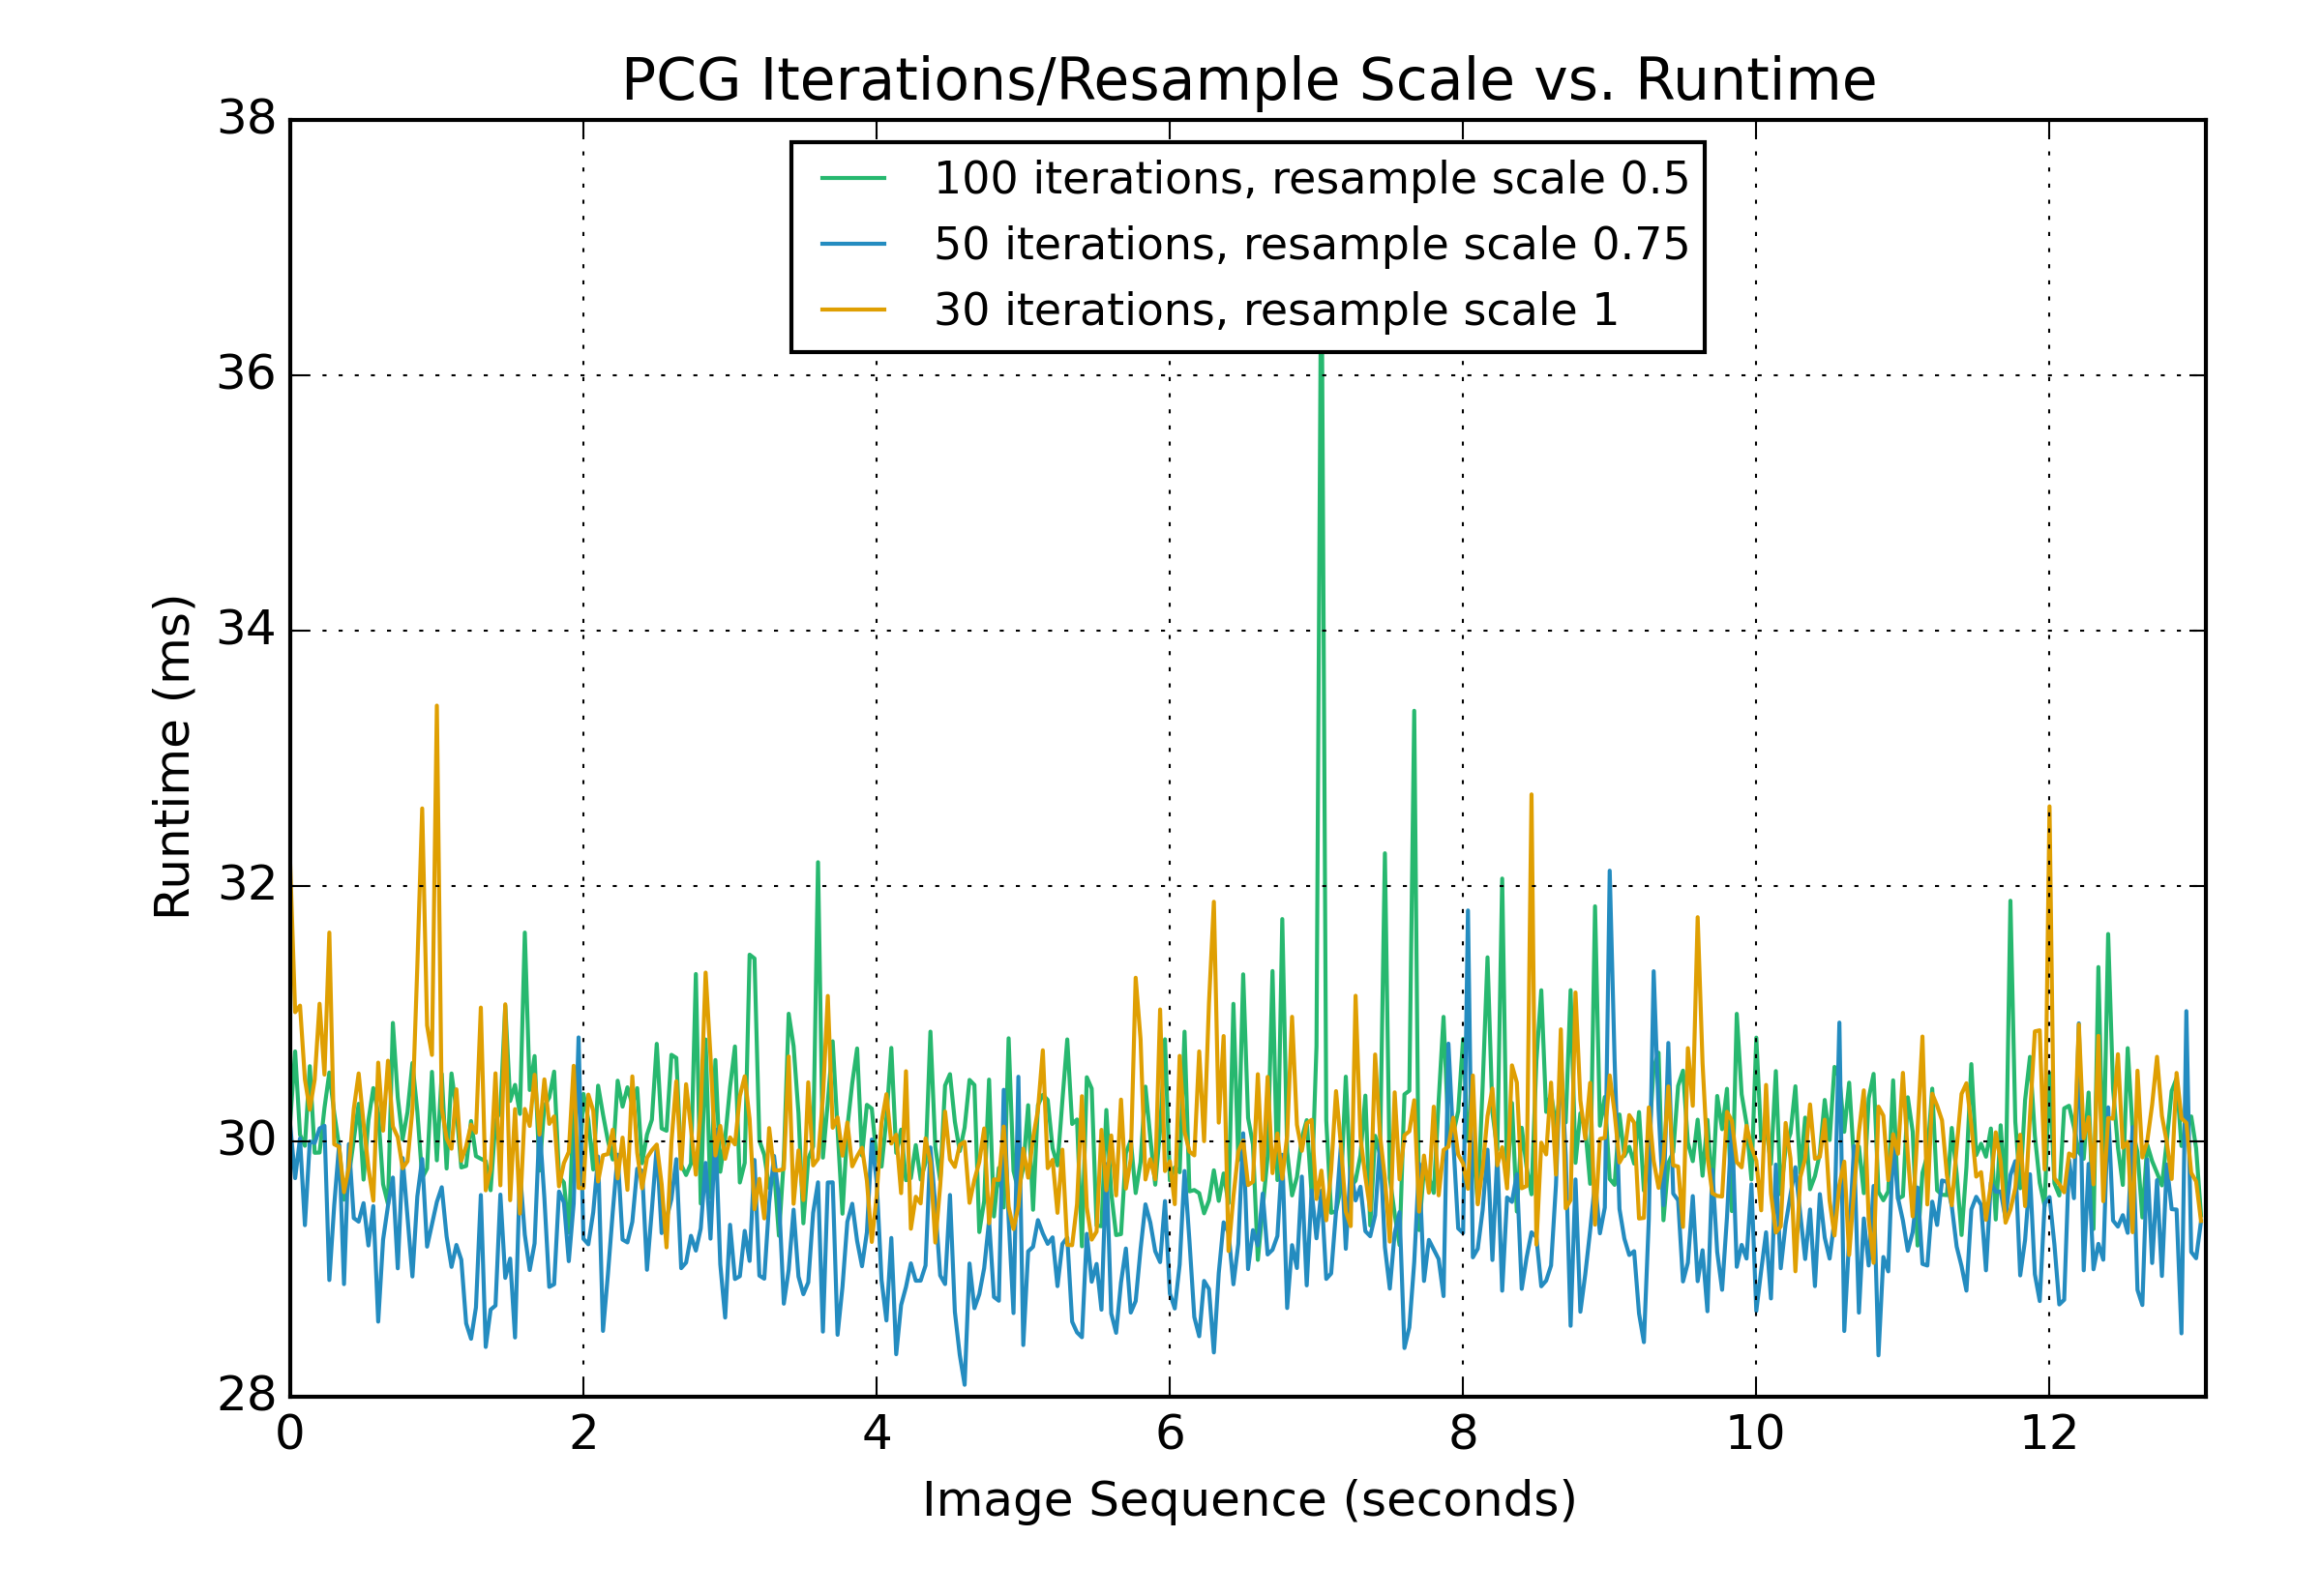
\includegraphics[width=0.75\textwidth]{{figures/cudacm/evaluation/runtime_30ms}.png}
	\caption{
		\textbf{Solver runtime per frame} for the kidney data set with different configurations of PCG iterations and resample scales targeting $30$ms per frame.
		Smaller images yield a smaller problem size and thus allow for a higher number of iterations.
	}
	\label{fig:cudacm:evaluation-30ms}
\end{figure}
As shown in Figure \ref{fig:cudacm:evaluation-30ms}, the image size has a significant impact on the runtime performance, since the problem size can be significantly reduced by resampling the ultrasound images to a smaller resolution, compute the corresponding Confidence Maps and then upsample the result to back the original resolution.
While our test platform allows for only $30$ PCG iterations in full resolution, $50$ iterations are feasible with a resample scale of $0.75$ in each direction and over $100$ iterations are possible with a resample scale of $0.5$ in each direction.
Though the frame rates are rather constant, a jitter in the computation times is present.
Therefore, we do not limit our incremental solver by the number of iterations but by a given time budget.


\paragraph{Resample Scale vs. Image Quality}
While it is no surprise that smaller images allow for a higher number of PCG iterations, the interesting question is what impact the downsampling has on the image quality of the computed Confidence Maps.
We use the Structured Similarity Index Measure (SSIM) with a window size of $9 \times 9$ pixels \cite{Wang:2004:SSIM} for a quantitative comparison of our results with the exact reference solution.
This \SYN{makes sense} since we intend to use our real-time uncertainty estimation framework mainly for visualization purposes.
By modeling perceptual effects through \SYN{comparing} the covariance between the two images with their individual variances, the SSIM provides an excellent quantitative assessment of the perceived image quality.

\begin{figure}[ht]
	\centering
	\subfloat[~Minimal SSIM per frame for kidney data set.]{
		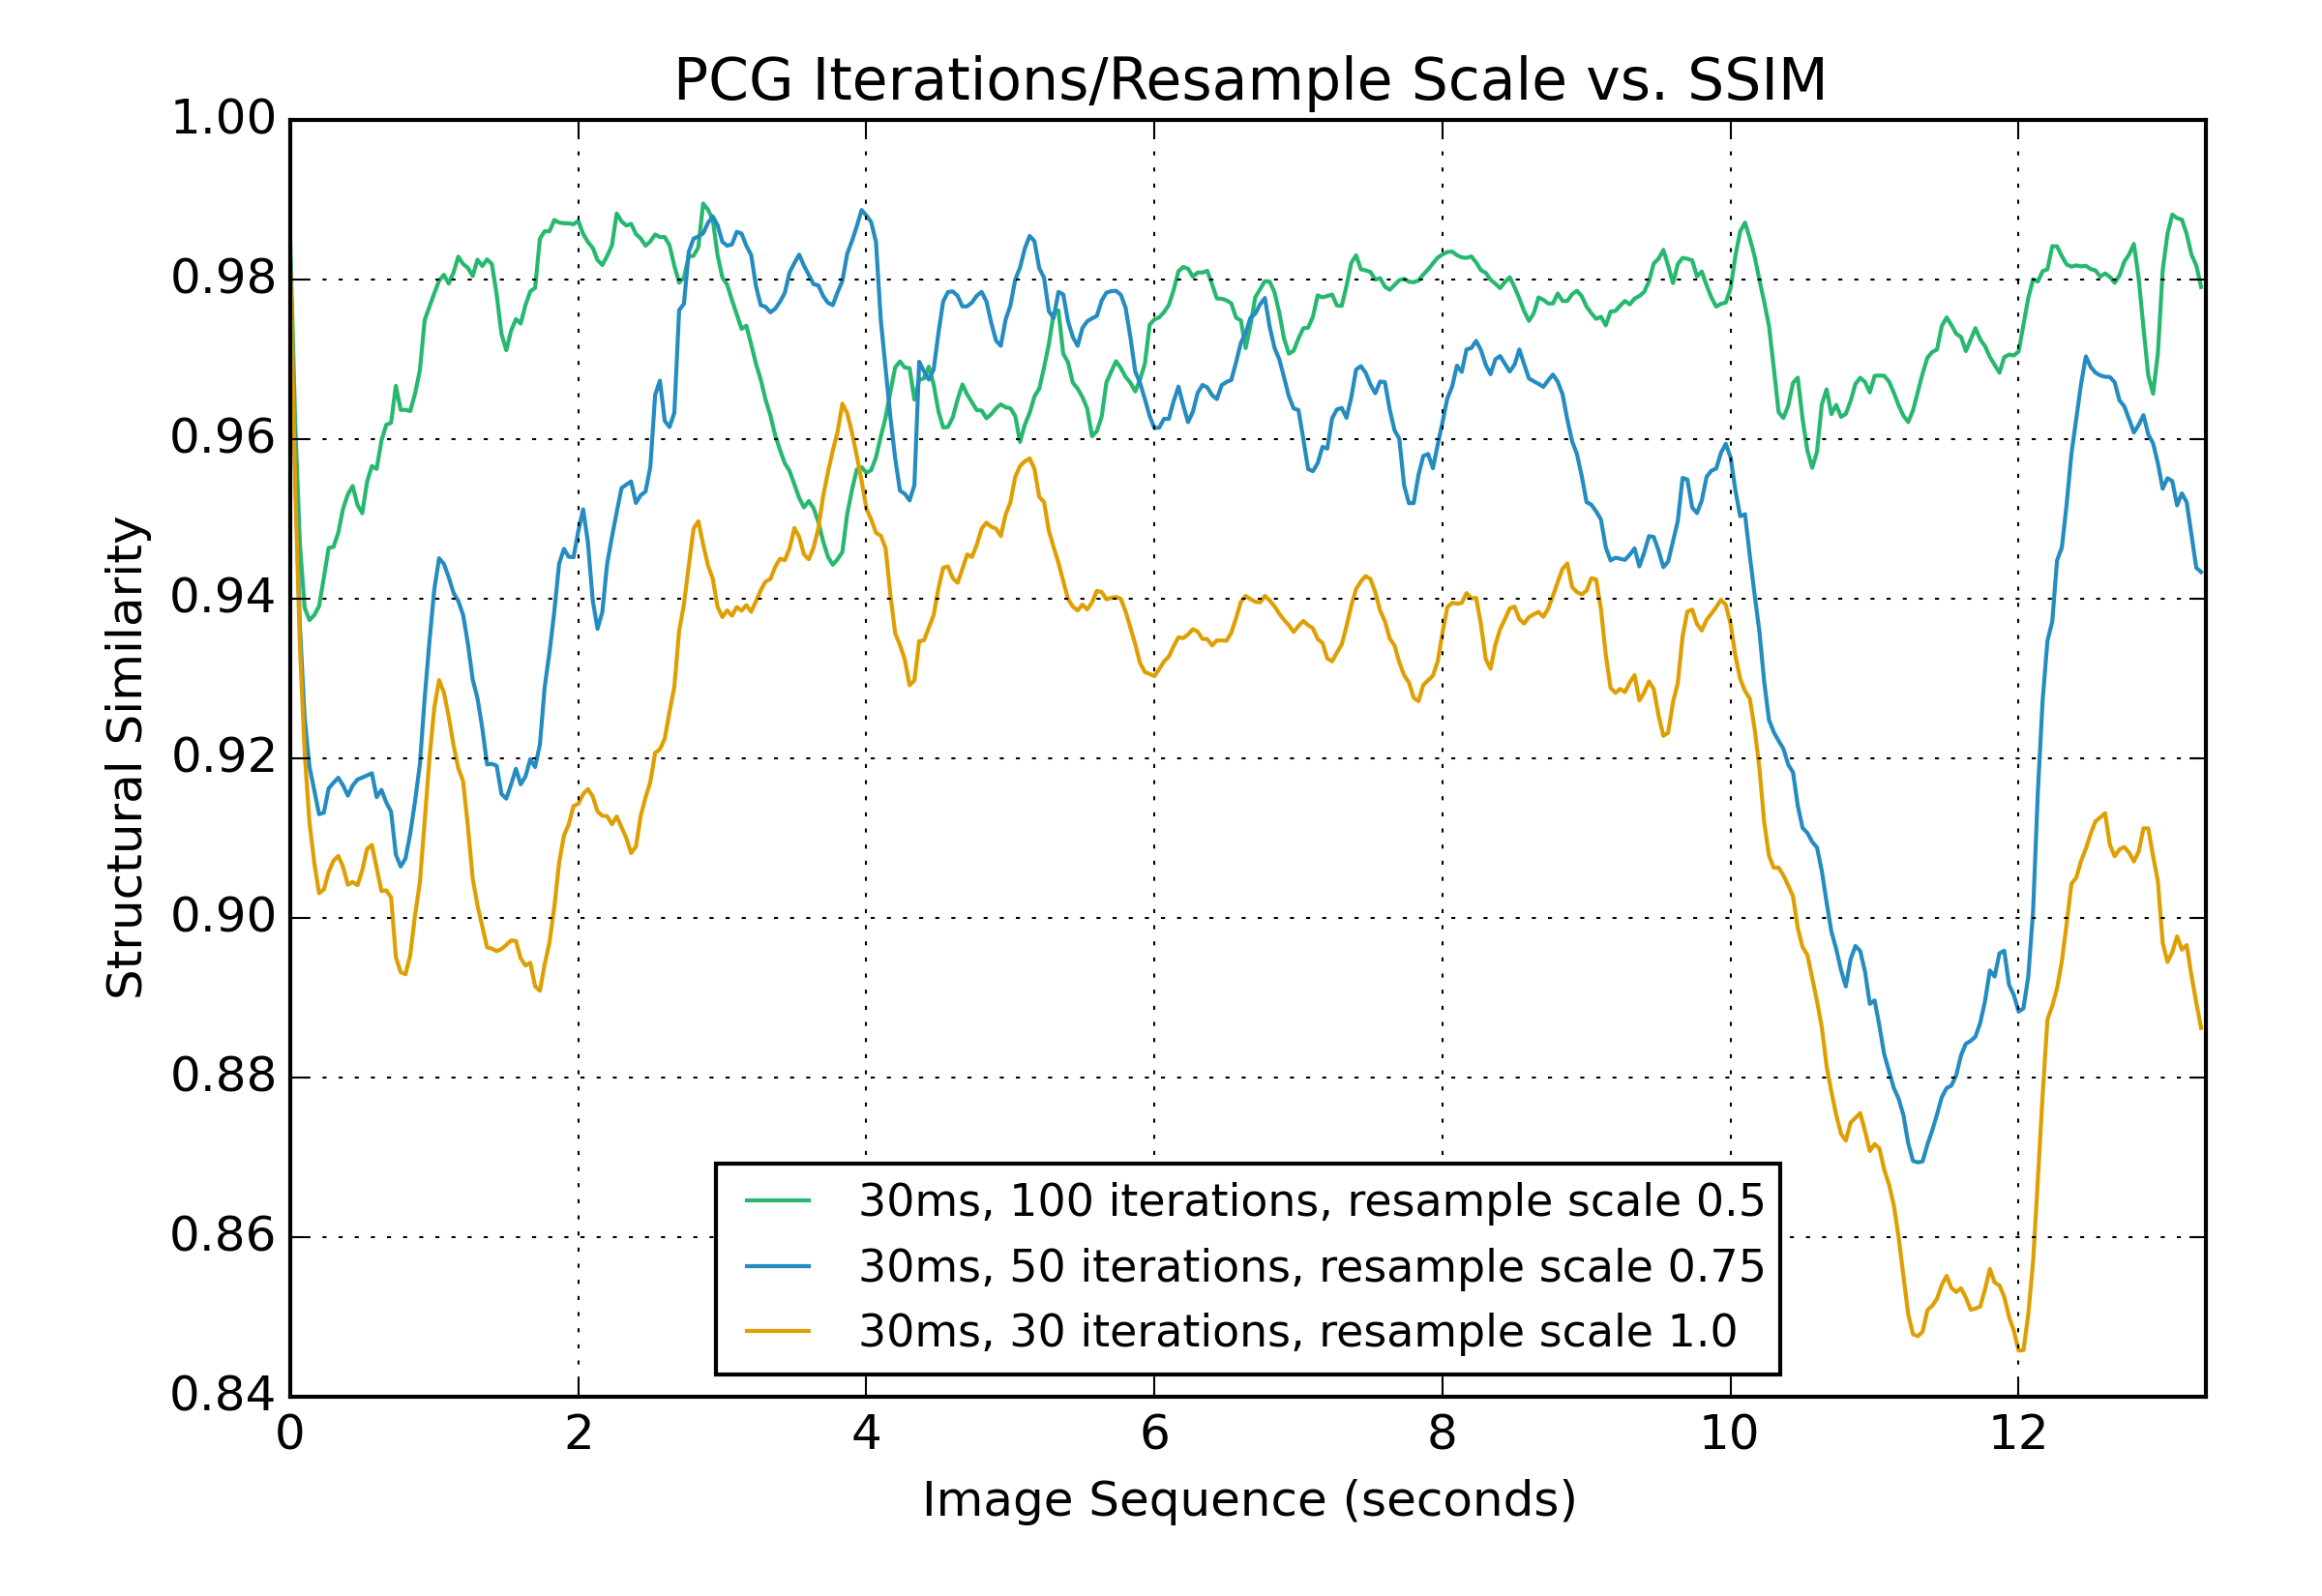
\includegraphics[width=0.49\textwidth]{figures/cudacm/evaluation/kidney_minssim_30ms.png}
	}
	\subfloat[~Minimal SSIM per frame for gullbladder data set.]{
		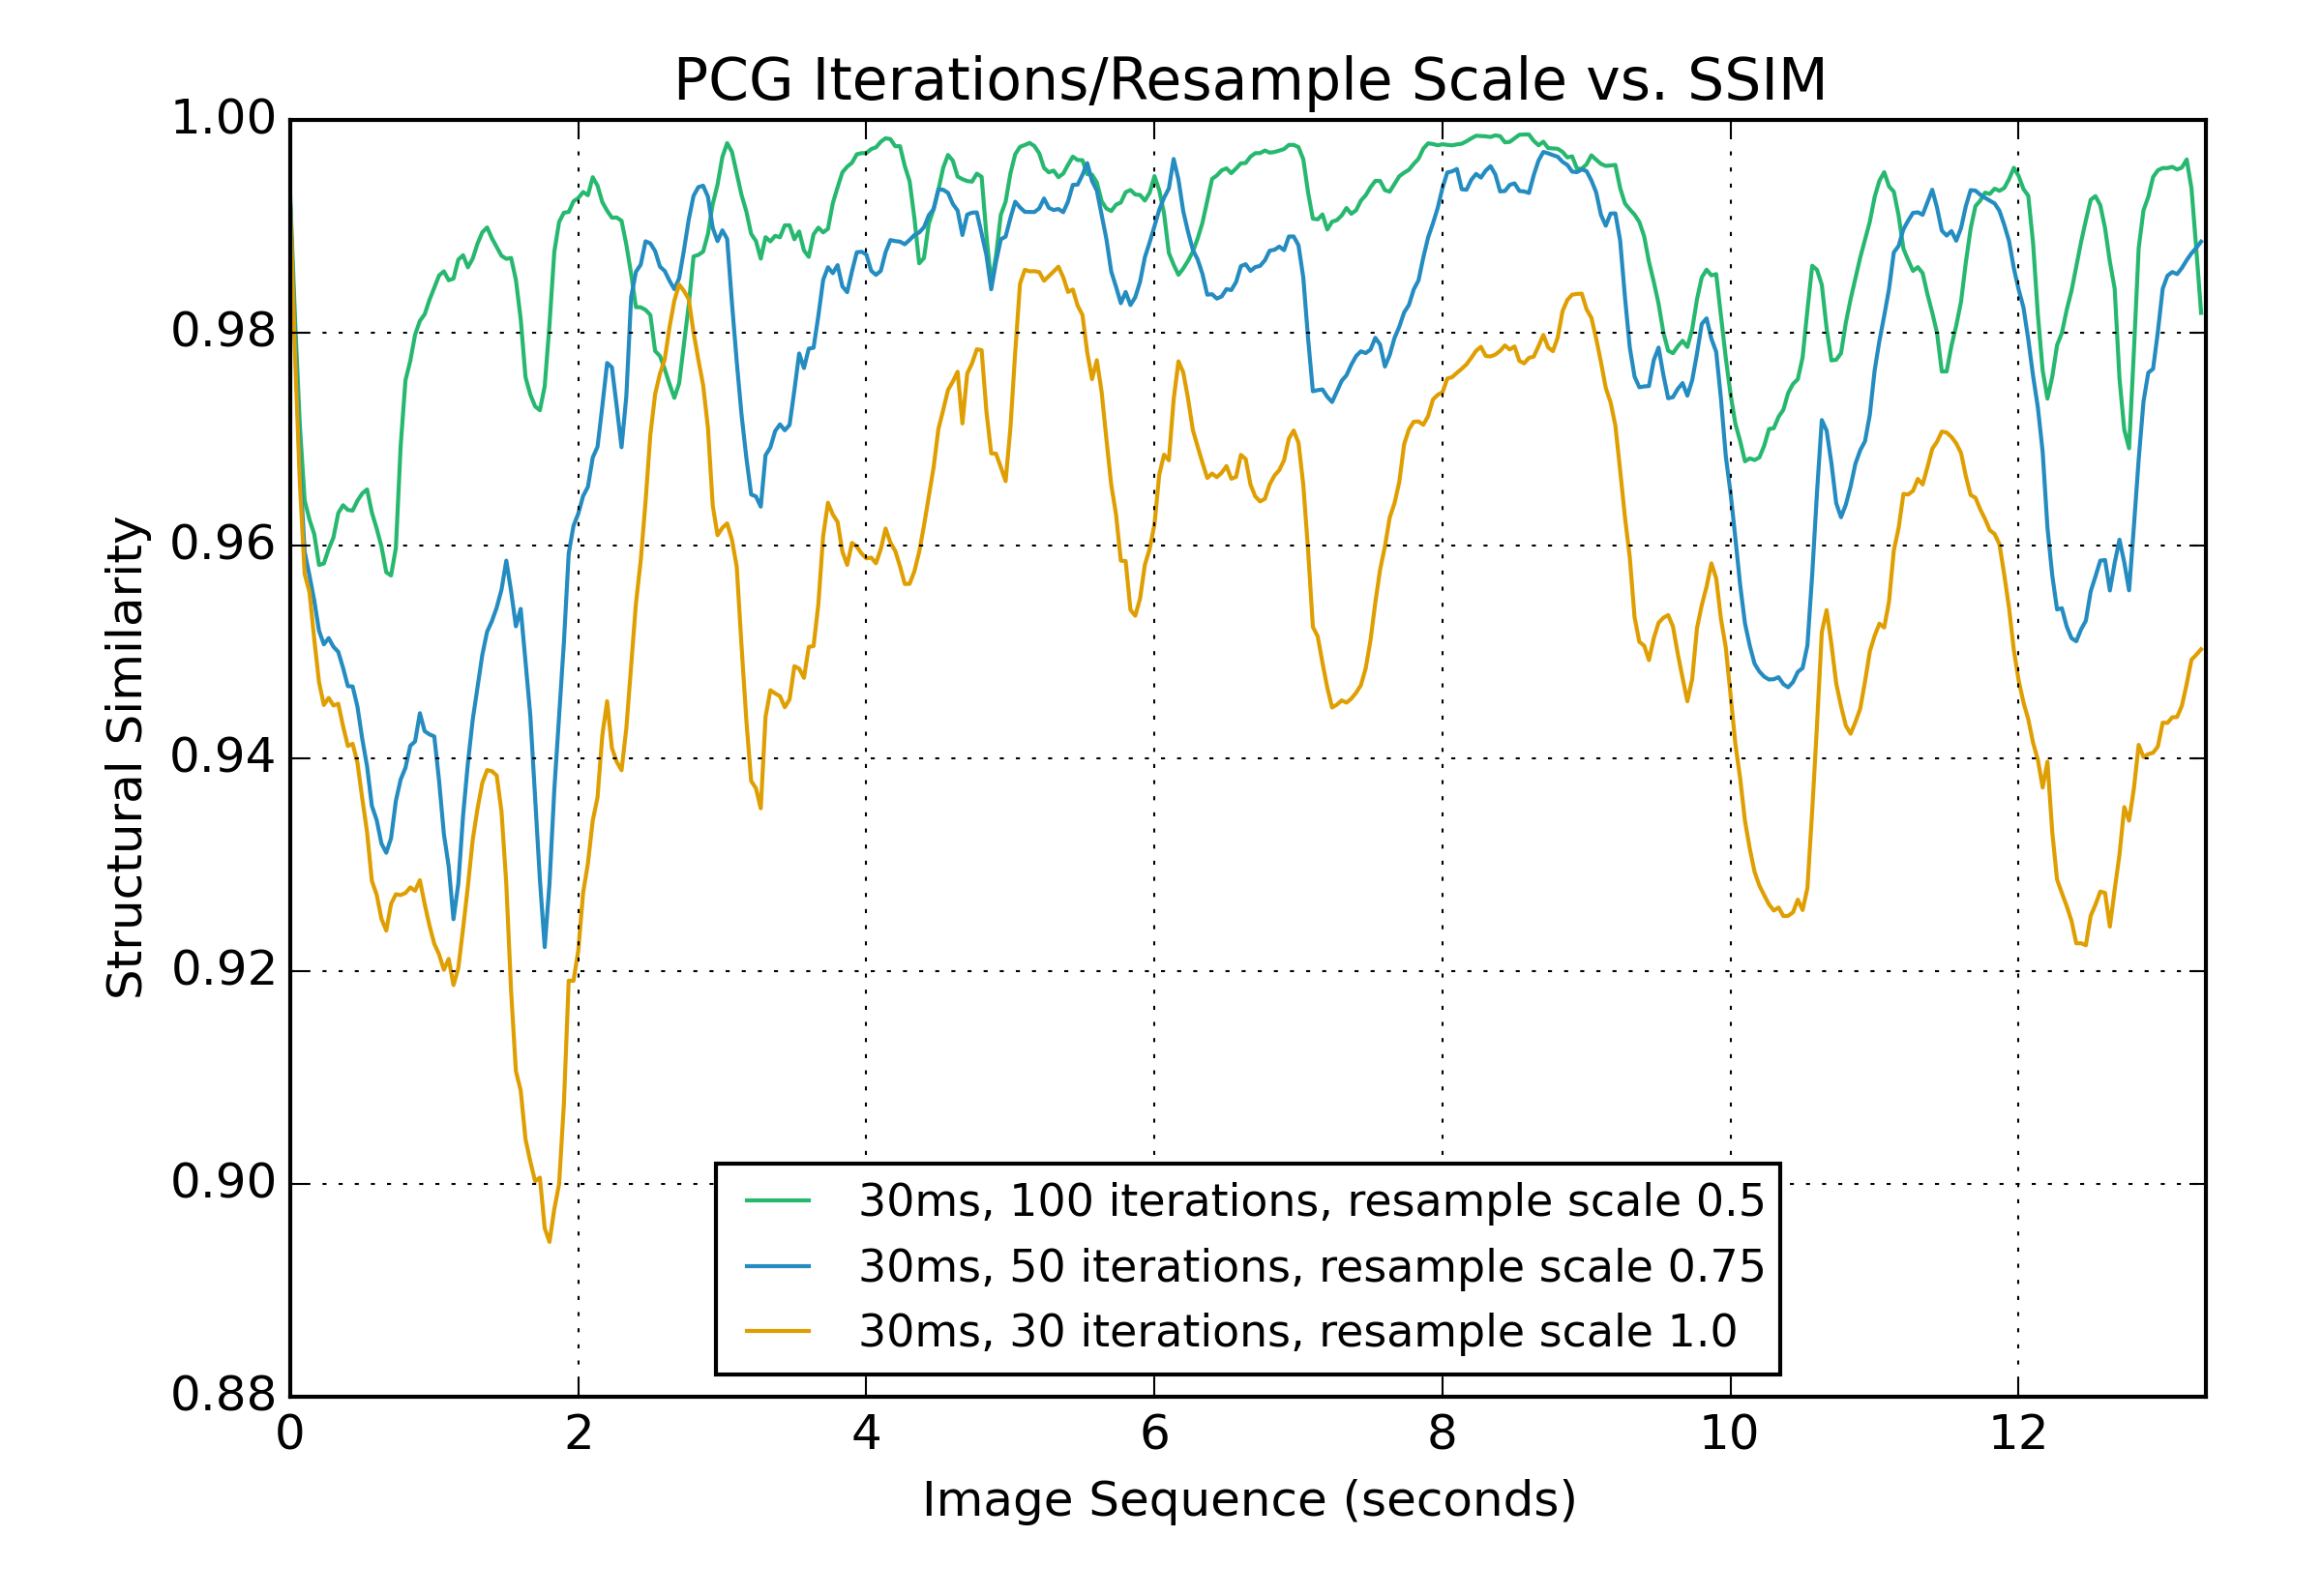
\includegraphics[width=0.49\textwidth]{figures/cudacm/evaluation/gullbladder_minssim_30ms.png}
	}
	\caption{
		Evaluation on the \textbf{image quality with respect to the resample scale} in terms of structural similarity.
		When maintaining a target time budget of 30ms, a lower resample scale yields a better image quality.
	}
	\label{fig:cudacm:evaluation-30ms-error}
\end{figure}

Smaller images exhibit both a smaller computational burden and a higher convergence rate of the solver, so that the resampling may even be beneficial for the resulting image quality.
However, at the same time, the lower resolution of the images may remove little details, which are important for the correct estimation of the signal attenuation.
When looking at Figure \ref{fig:cudacm:evaluation-30ms-error}, one can see that in general a slight downsampling of the images is benefitial for the final image quality.
For a couple of frames however, in particular with the kidney data set, details get lost yielding a worse structural similarity applying less PCG iterations on the full scale images.
With these results, we decided that using a resample scale of $0.5$ defines a good trade-off between computation time and image quality (cf. Figure \ref{fig:cudacm:evaluation-30ms-error}).


\paragraph{PCG Iterations vs. Image Quality}
As a final quantitative evaluation, we ran our proposed solver scheme with a fixed resample scale of $0.5$ but different number of iterations.
As illustrated in Figure \ref{fig:cudacm:performance_evaluation}, the SSIM never falls below $0.94$ when performing $110$ PCG iterations, which is an excellent result.
\begin{figure}[ht]
	\centering
	\subfloat[~Minimal SSIM per frame for kidney data set.]{
		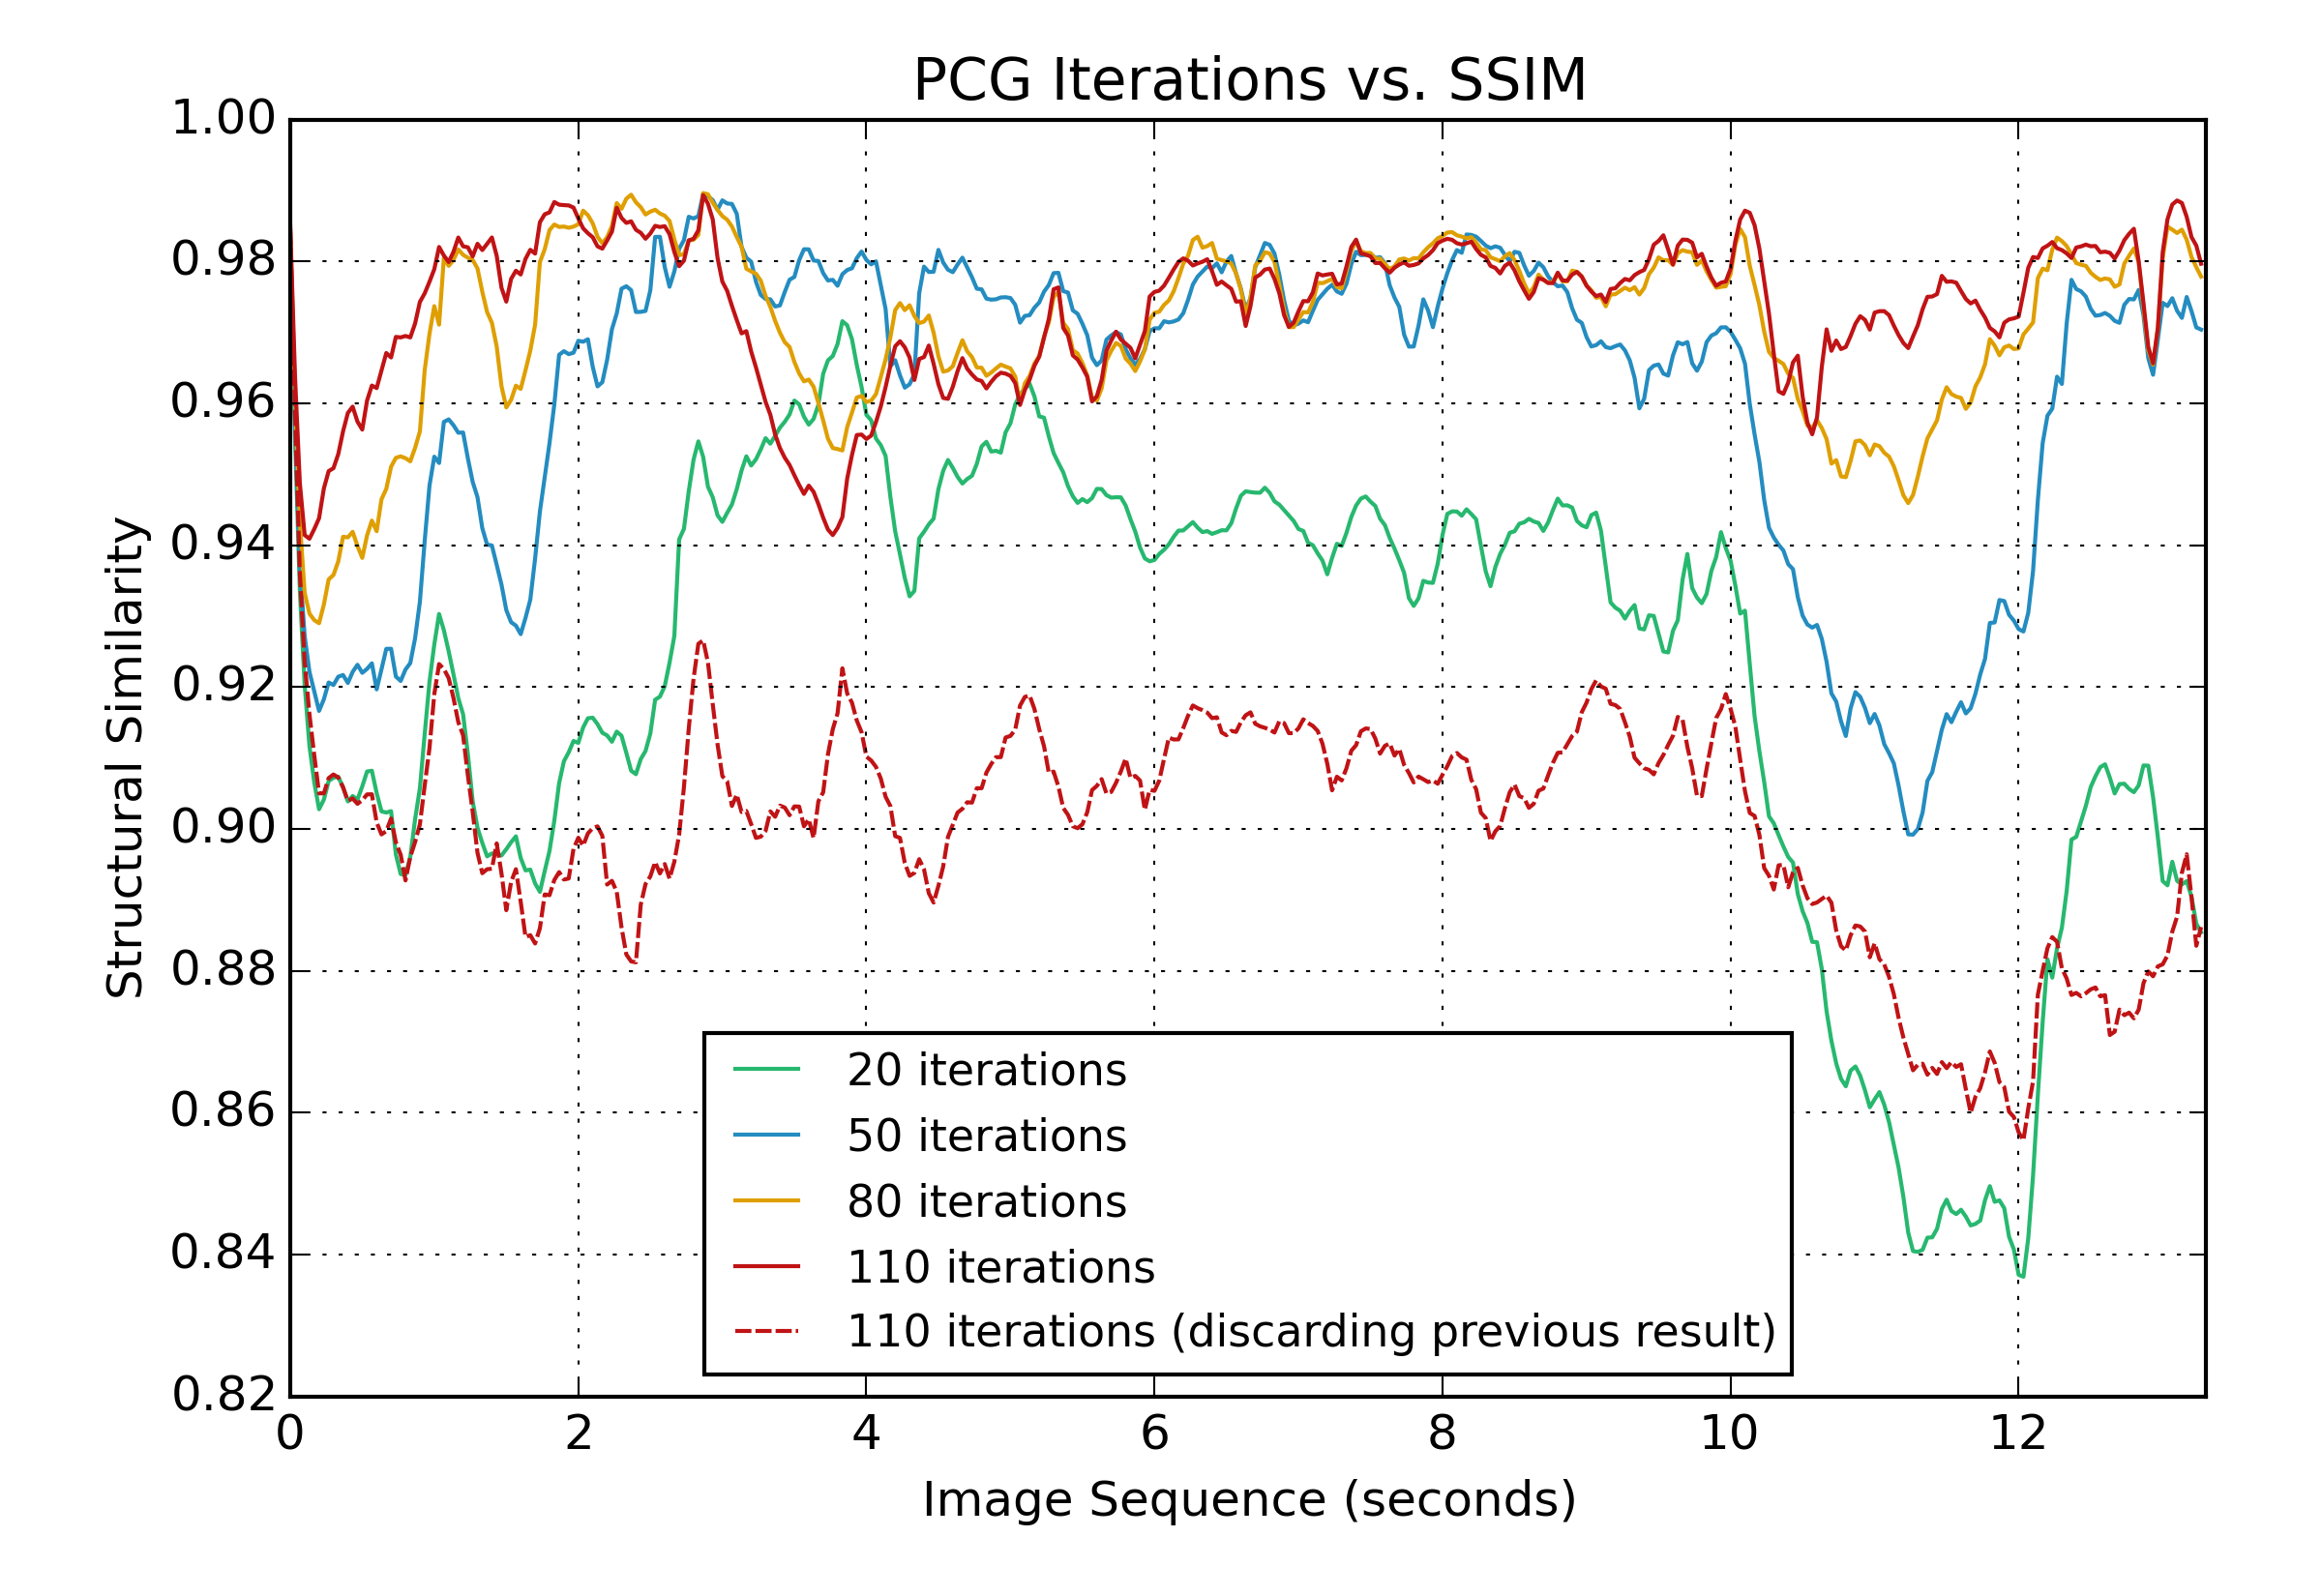
\includegraphics[width=0.49\textwidth]{{figures/cudacm/evaluation/kidney_iterations_vs_minssim_0.50}.png}
	}
	\subfloat[~Minimal SSIM per frame for gullbladder data set.]{
		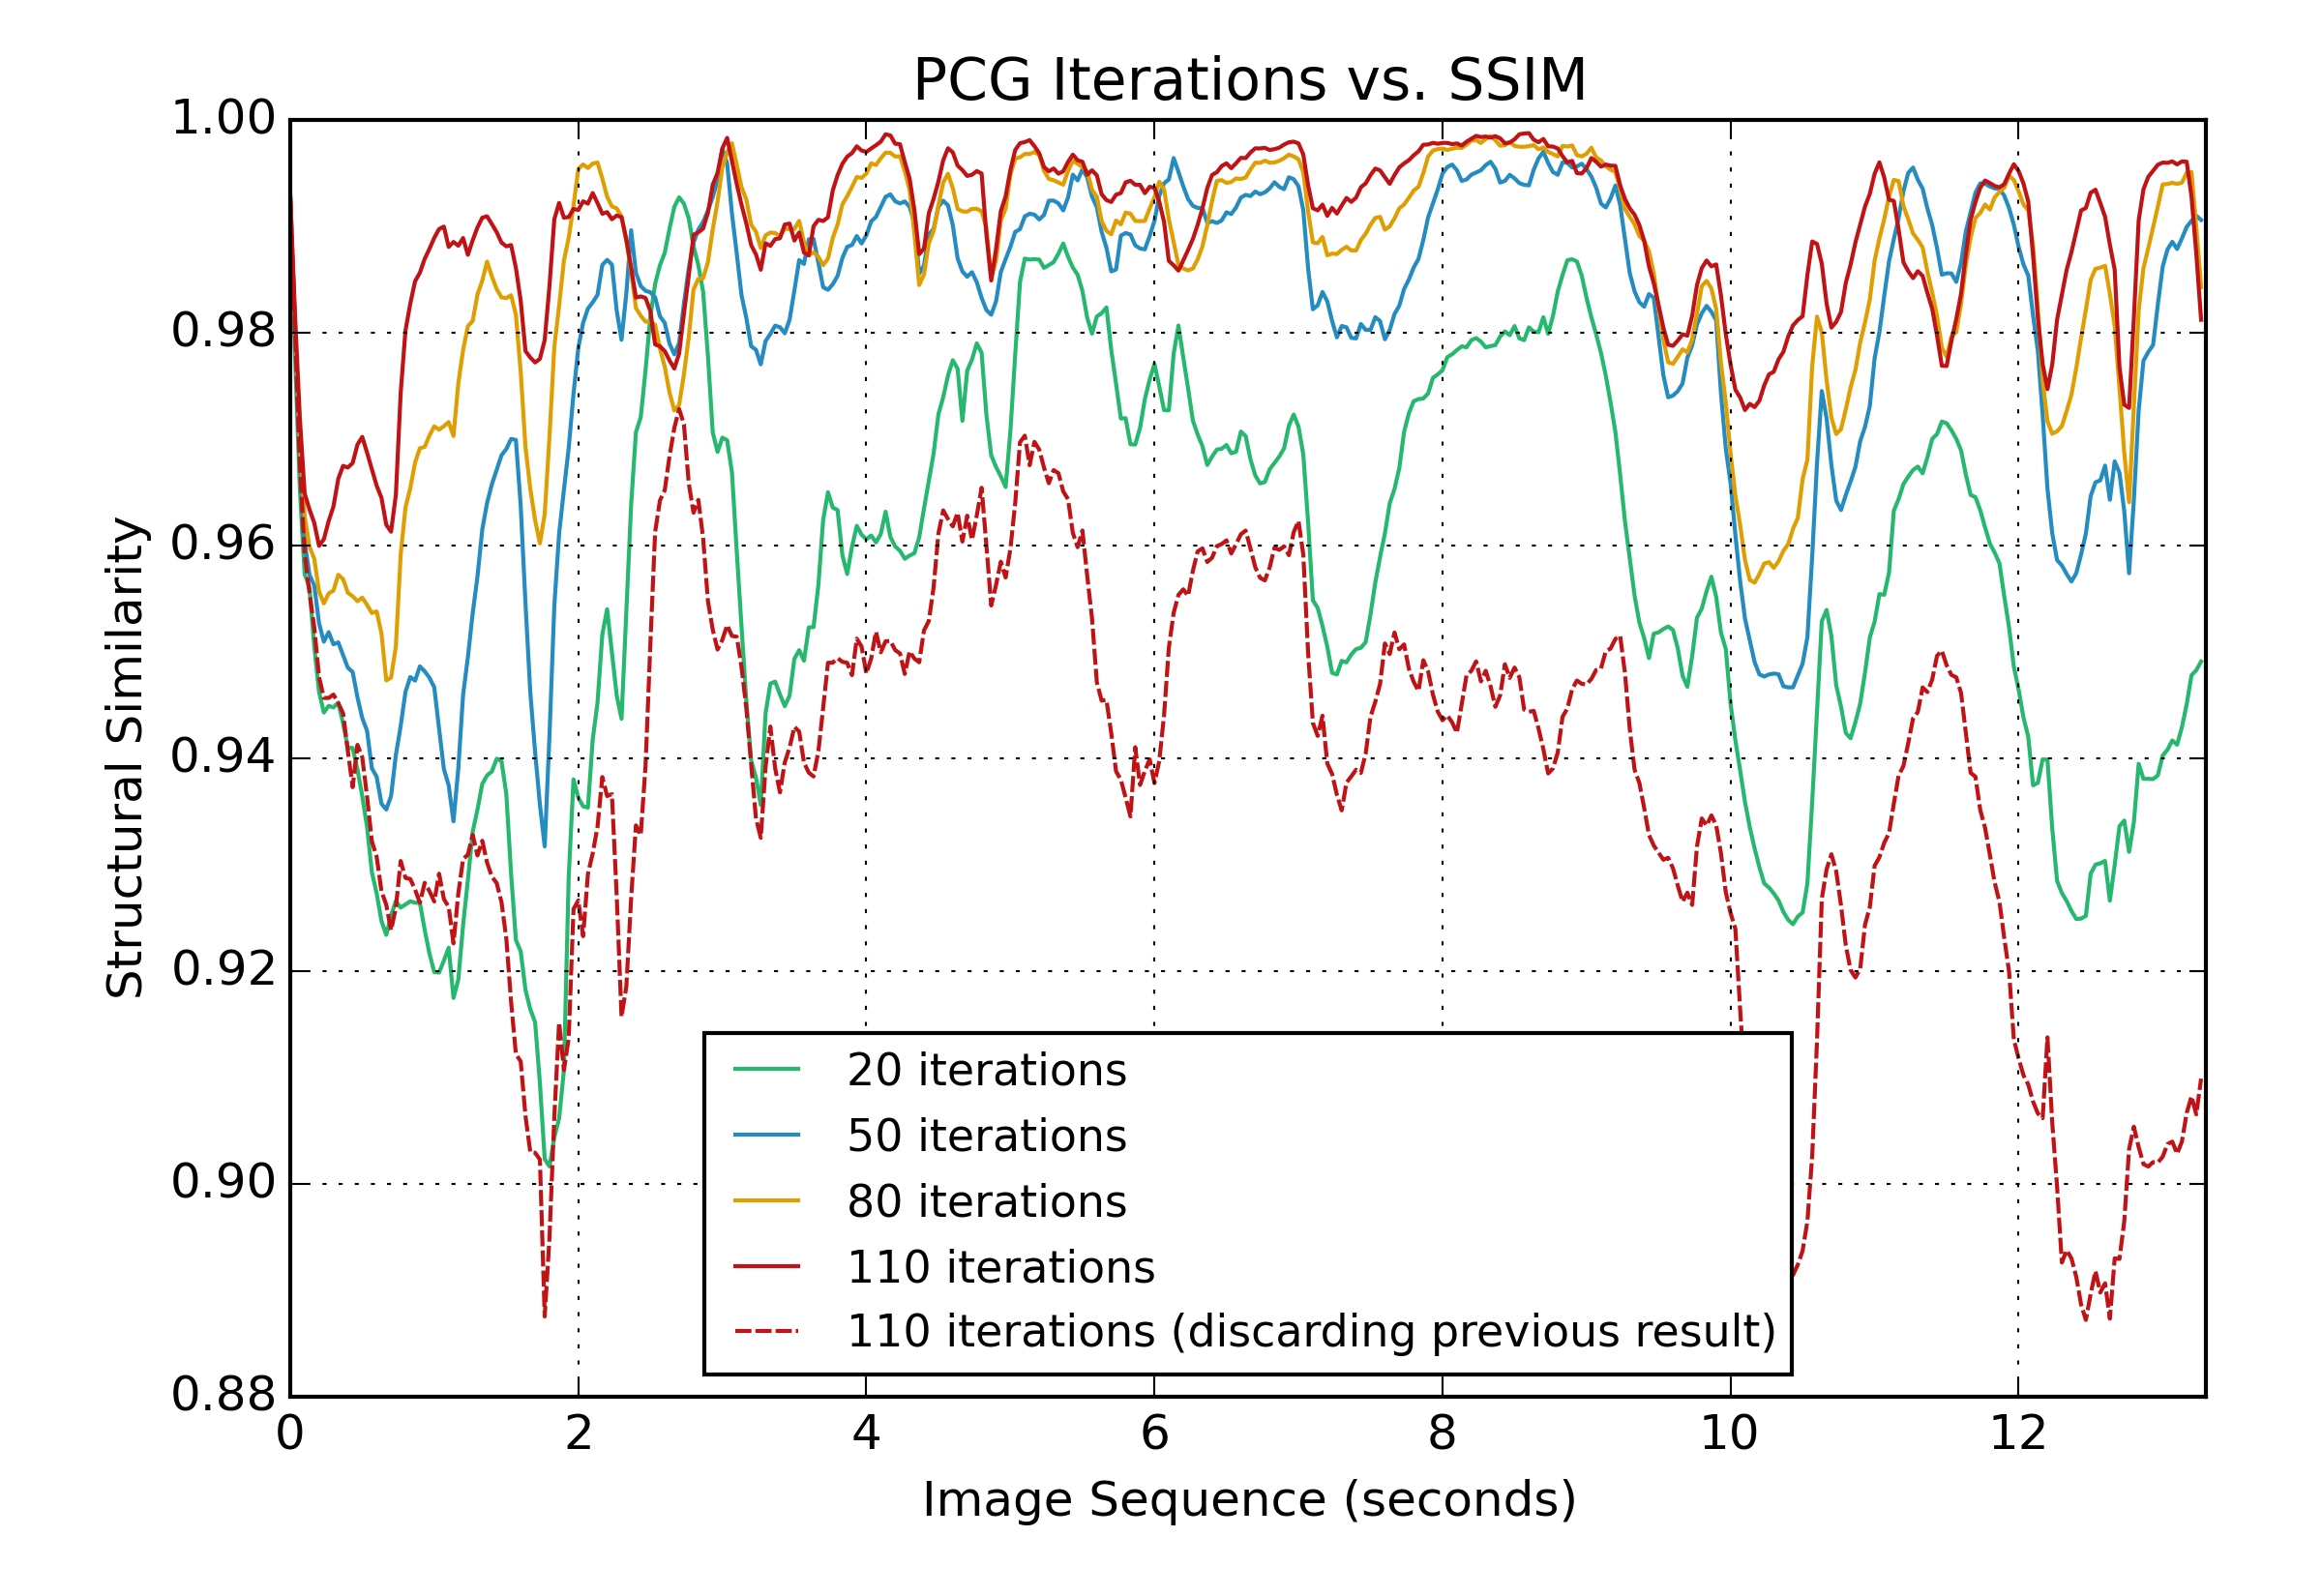
\includegraphics[width=0.49\textwidth]{{figures/cudacm/evaluation/gullbladder_iterations_vs_minssim_0.50}.png}
	}
	\caption{
		\textbf{Error (residual norm) over time} for different PCG iteration counts. 
		The resample scale was fixed to 0.5.
	}
	\label{fig:cudacm:performance_evaluation}
\end{figure}
For comparison, the dashed lines show the error progression when the solver is reinitialized at each iteration, which yields mostly worse results than 20 incremental iterations.
This demonstrates the importance of leveraging the dynamic nature of ultrasound and the effectiveness of our technique using the solution of the previous frame as initialization.
Table \ref{tbl:cudacm:kidney-results} further summarizes the results and shows the average runtime, average SSIM and minimum SSIM over the entire kidney data set.
One can see that the $110$ incremental PCG iterations of our reference implementation are real-time capable and yielding almost exact results with an average SSIM of $0.999$ and a minimum SSIM of only $0.941$.
Figure \ref{fig:cudacm:kidney-qualitative} presents qualitative results on a representative frame of the same ultrasound sequence.

\begin{table}[ht]
	\centering
	\begin{tabu} to 0.9\linewidth {>{\bfseries\centering}m{35mm} C C C}
		\toprule
		\multirow{2}{*}{\# Iterations} & \ \bfseries Avg. Runtime \ & \bfseries Avg. Quality & \bfseries Min. Quality    \\
		                               & \ \emph{(ms)} \            & \multicolumn{2}{c}{\emph{(Structural Similarity)}} \\
		\midrule
		Direct solver                  & \ $2214.68$ \              & \ $1.0$ \              & \ $1.0$ \                 \\
		\midrule
		20 (incremental) \             & \ $10.84$ \                & \ $0.991$ \            & \ $0.837$ \               \\
		50 (incremental) \             & \ $18.07$ \                & \ $0.997$ \            & \ $0.899$ \               \\
		80 (incremental) \             & \ $25.37$ \                & \ $0.998$ \            & \ $0.929$ \               \\
		110 (incremental) \            & \ $32.46$ \                & \ $0.999$ \            & \ $0.941$ \               \\
		\midrule
		110 (discarding) \             & \ $32.59$ \                & \ $0.984$ \            & \ $0.856$ \               \\
		\bottomrule
	\end{tabu}
	\caption{
		Aggregated \textbf{performance results in terms of runtime an error} with different configurations for the number of iterations. 
		The resample scale was fixed to 0.5. 
		Data set was a patient kidney ultrasound sequence containing a total of 392 frames.
	}
	\label{tbl:cudacm:kidney-results}
\end{table}

\begin{figure}[p]
	\centering
	\subfloat[~Original ultrasound frame from kidney sequence.]{
		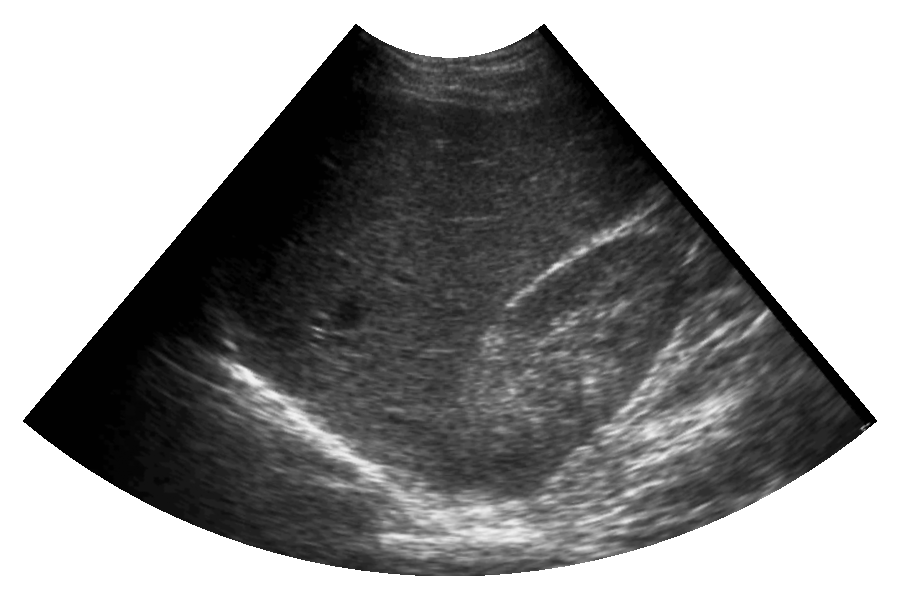
\includegraphics[width=0.46\textwidth]{figures/cudacm/evaluation/cm_stuff/329_us.png}
	}
	\quad
	\subfloat[~Corresponding Confidence Map.]{
		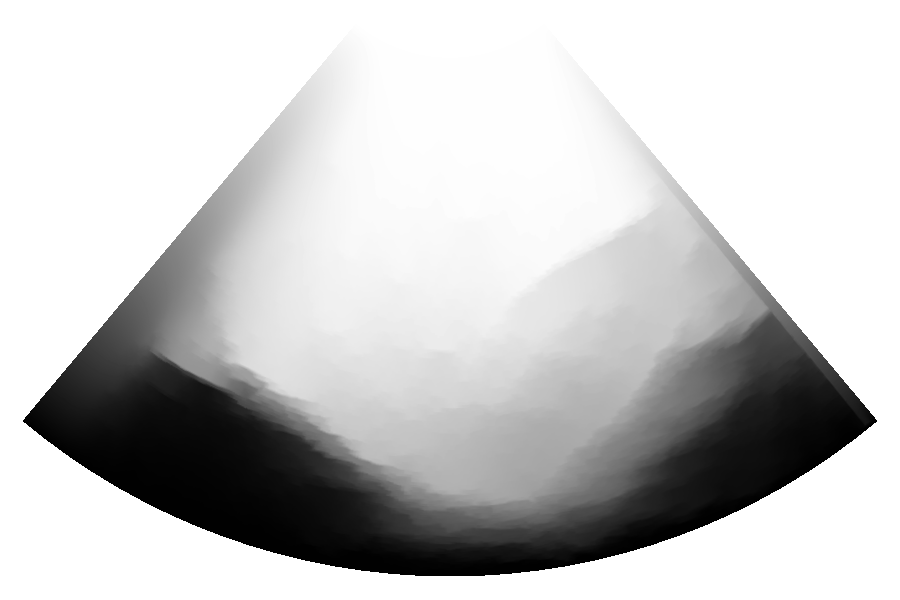
\includegraphics[width=0.46\textwidth]{figures/cudacm/evaluation/cm_stuff/329_512_5000_cm.png}
	} 
	\\
	\subfloat[~Computed Confidence Map with 30 iterations in full resolution ($30$ms).]{
		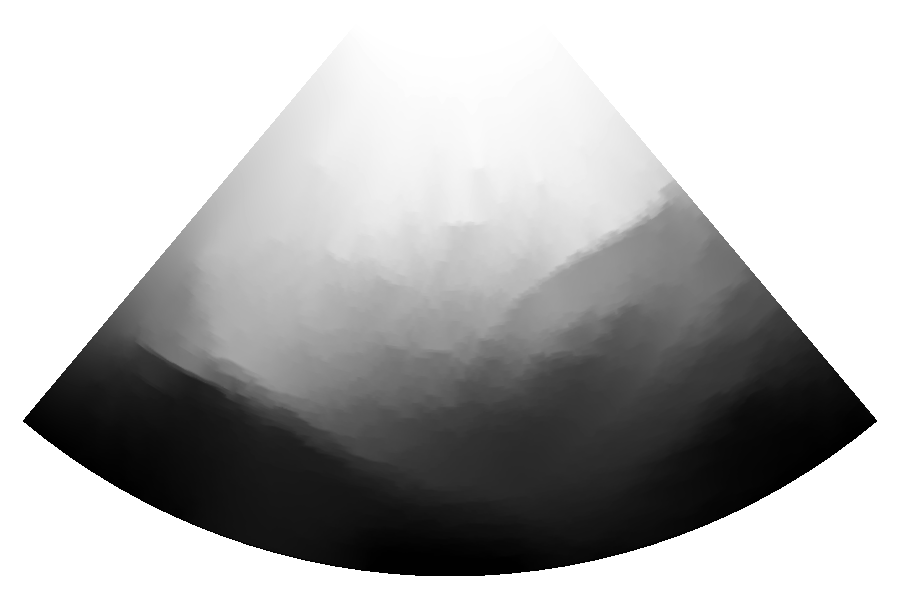
\includegraphics[width=0.46\textwidth]{figures/cudacm/evaluation/cm_stuff/329_512_30_cm.png}
	}
	\quad
	\subfloat[~Structured Similarity between (b) and (c); average: $0.984$, minimum: $0.889$.]{
		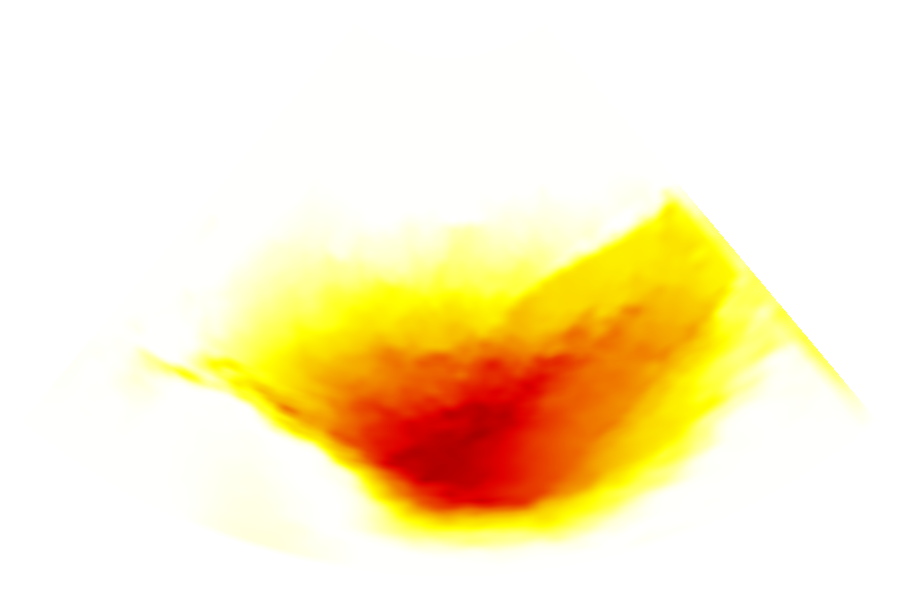
\includegraphics[width=0.46\textwidth]{figures/cudacm/evaluation/cm_stuff/329_512_30_ssim.png}
	}
	\\
	\subfloat[~Computed Confidence Map with 100 iterations in half resolution ($30$ms).]{
		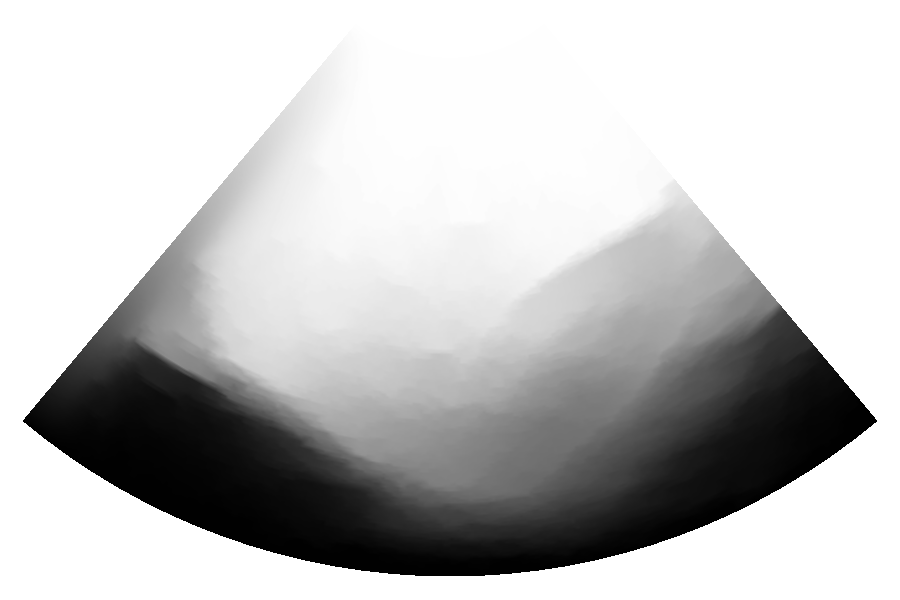
\includegraphics[width=0.46\textwidth]{figures/cudacm/evaluation/cm_stuff/329_256_110_cm.png}
	}
	\quad
	\subfloat[~Structured Similarity between (b) and (e); average: $0.998$, minimum: $0.973$.]{
		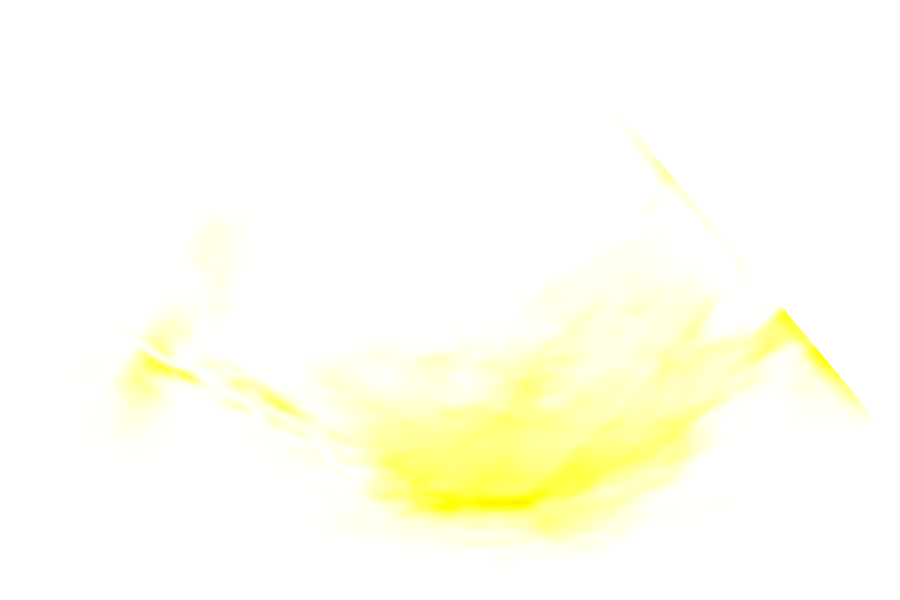
\includegraphics[width=0.46\textwidth]{figures/cudacm/evaluation/cm_stuff/329_256_110_ssim.png}
	} \\
	\caption{
		\textbf{Qualitative results of the presented incremental solver scheme}.
		By comparing (b) with (c) and (e), one can see the impact of the limited amount of iterations on the resulting Confidence Maps.
		The SSIM in (d) and (f) quantifies the perceptual difference.
		For better visualization of differences, the color map in (d) and (f) was normalized to the range of $[0.85, 1.0]$ and does not show the full SSIM range of $[-1, 1]$.
	}
	\label{fig:cudacm:kidney-qualitative}
\end{figure}


\section{Conclusion}
%\TODO{Write a conclusion for this chapter}
We presented a method to bring the estimation of B-mode ultrasound signal attenuation into real-time applications.
Building on ultrasound Confidence Maps, originally proposed by Karamalis et al. \cite{Karamalis:2012:ConfidenceMaps}, we propose an incremental solver scheme, which leverages the temporal coherency of ultrasound imaging.
In an extensive evaluation with clinical patient data, we assessed the impact of our different optimizations on the quality of the computed Confidence Maps and showed that our methods yield accurate approximations within a $30$ms time budget.
In the remainder of this thesis, we will use this work to generate real-time uncertainty informations for different ultrasound processing and visualization techniques.
